% ---------------- Beginn Präambel --------------

% Datum: 06.11.2023
% Vorname: Daniel 
% Nachname: Bading
% Matrikelnummer: 405020
% E-Mail: daniel.bading@campus.tu-berlin.de

% ---------------- Ende Präambel --------------

\documentclass{scrartcl} 

\usepackage[utf8]{inputenc}
\usepackage[english]{babel}
\usepackage{amsmath, amssymb, amsthm, mathtools}
\usepackage{makecell} % damit man in der Tabelle die erste Zeile spalten kann
\usepackage{graphicx} % damit man Bilder einfügen kann
\usepackage{subcaption} % damit man in einer figure-Umgebung mehrere figures einbinden kann
\usepackage{float} % damit die Abbildung auch exakt da ist, wo man sie im Text einbinden will
\usepackage{tikz}
\usepackage[miktex]{gnuplottex}
\usepackage{listings}

%\graphicspath{ {./images/} } % hier lässt sich auch einfach der Weg zu dem Ordner speichern, sodass die Bilder nicht im gleichen Verzeichnis liegen müssen

\title{Hausaufgabe 2 - Einführung in Latex}
\author{
  Bading, Daniel\\
  \texttt{daniel.bading@campus.tu-berlin.de}\\
  Matrikelnummer: 405020
  }
\vfill
\date{\today}
  
\begin{document}

\maketitle

\newpage

\tableofcontents

\newpage

% ------------ Beginn eigentlicher Text ---------

\section{Hausaufgabe 5.1}

\begin{table}[h]
\label{tab:planeteninfos}
\captionabove{Planeteninformationen}
\centering
\begin{tabular}{| l | c | c | c | }
\hline
\textbf{Planet} & \thead{Abstand Erde \\ (Mio. km)} & \thead{Abstand Sonne \\ (Mio. km)} & \textbf{Masse (kg)} \\ 
\hline
Merkur & 77.3 & 57.9 & \(3.30 \times 10^{23}\) \\
Venus & 38.2 & 108.2 & \(4.87 \times 10^{24}\) \\
Erde & 0 & 149.6 & \(5.97 \times 10^{24}\) \\
Mars & 78.3 & 227.9 & \(6.39 \times 10^{23}\) \\
Jupiter & 629.0 & 778.5 & \(1.90 \times 10^{27}\) \\
Saturn & 1,269.0 & 1,427.0 & \(5.68 \times 10^{26}\) \\
Uranus & 2,550.0 & 2,870.0 & \(8.68 \times 10^{25}\) \\
Neptun & 4,303.0 & 4,504.0 & \(1.02 \times 10^{26}\) \\
\hline
\end{tabular}
\end{table}

Unsere faszinierende Nachbarschaft im Sonnensystem besteht aus verschiedenen Planeten, von denen jeder seine einzigartigen Eigenschaften besitzt. Der sonnennächste Planet, Merkur, rast mit beeindruckenden 57.9 Millionen Kilometern pro Stunde um die Sonne, während die Venus mit ihrem dichten Atmosphärenschleier den zweiten Platz einnimmt. Die Erde, unsere Heimat, ruht im gemütlichen Abstand von 149.6 Millionen Kilometern von der Sonne und beherbergt eine Vielfalt von Lebensformen. \\
\\
Mars, auch als der Rote Planet bekannt, steht stolze 78.3 Millionen Kilometer von der Erde entfernt. In seinem ständigen Streben nach Entdeckung schickt die Menschheit Raumsonden, um das Geheimnis seiner Oberfläche zu ergründen. Jupiter, der Riese des Sonnensystems, beeindruckt nicht nur durch seine massive Größe, sondern auch durch seine imposanten 778.5 Millionen Kilometer Abstand zur Sonne.\\
\\
In den äußeren Regionen des Sonnensystems finden wir die Gasriesen Saturn, Uranus und Neptun. Saturn, mit seinem atemberaubenden Ringsystem, schwebt majestätisch 1,269 Milliarden Kilometer von der Sonne entfernt. Uranus, der aufgrund seiner Seitenlage als "liegender Planet" bekannt ist, liegt 2,550 Milliarden Kilometer von der Sonne entfernt. Neptun, der äußerste bekannte Planet, befindet sich atemberaubende 4,303 Milliarden Kilometer von der Sonne entfernt und schwingt in tiefem Blau durch das äußere Sonnensystem. \\
\\
Diese Zahlen, die in der Tabelle \ref{tab:planeteninfos} dargestellt werden, verdeutlichen die enorme Vielfalt und die erstaunlichen Entfernungen, die die Planeten voneinander und von der Sonne trennen, und lassen uns ehrfürchtig über die Schönheit und Komplexität unseres Sonnensystems nachdenken.

\newpage
\section{Hausaufgabe 5.2}

\begin{figure}[h]
\centering
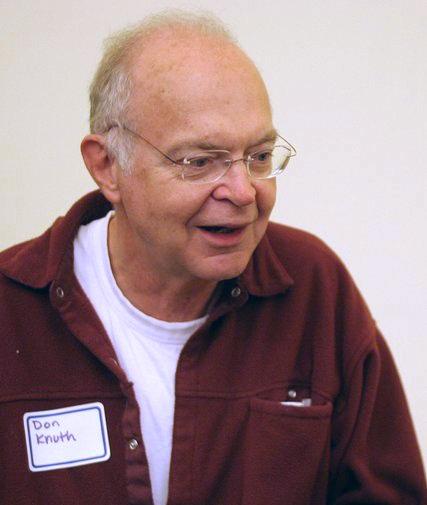
\includegraphics[scale=.5]{bild1.jpg}
\caption{Donald Knuth}
\label{fig:donknuth}
\end{figure}

Donald Ervin Knuth (Abbildung~\ref{fig:donknuth}), geboren am 10. Januar 1938, ist ein angesehener amerikanischer Informatiker und emeritierter Professor an der Stanford University. Er ist besonders bekannt für seine bedeutenden Beiträge zur Informatik und seine herausragenden Schriften im Bereich der Algorithmen und Computerprogrammierung.  Knuth ist am besten für sein mehrbändiges Werk "The Art of Computer Programming" bekannt, das als eine der umfassendsten und einflussreichsten Ressourcen im Bereich der Algorithmik gilt. In diesem Werk hat er nicht nur Algorithmen detailliert beschrieben, sondern auch einen einzigartigen Schreibstil kultiviert, der von vielen bewundert wird.  Ein weiterer herausragender Beitrag von Knuth ist das Textsatzsystem TeX, das er entwickelte, um mathematische und wissenschaftliche Dokumente typografisch ansprechend zu setzen. LaTeX, ein auf TeX basierendes System, wird weltweit von Wissenschaftlern und Autoren verwendet.  Don Knuth hat zahlreiche Auszeichnungen für seine Arbeit erhalten, darunter den Turing Award, der als höchste Auszeichnung in der Informatik gilt. Neben seiner akademischen Tätigkeit ist er auch für seine Hingabe an handgeschriebene Bücher und seine Betonung von Präzision und Schönheit in der Programmierung bekannt. Knuth bleibt eine inspirierende Figur und eine Schlüsselfigur in der Geschichte der Informatik.\\
\\
Nun wollen wir eine \texttt{figure}-Umgebung erstellen, in der wir zwei \texttt{subfigures} erstellen, wo wir dann bild2.jpg und bild3.png einfügen wollen. Es lässt sich die Größe oder Width der \texttt{figure} auf 90\% einstellen, sodass bei den bildern nichtmehr auf die skalierung geachtet werden muss. \\

\begin{figure}[H]
%\centering
\begin{subfigure}{.45\textwidth}
  \centering
  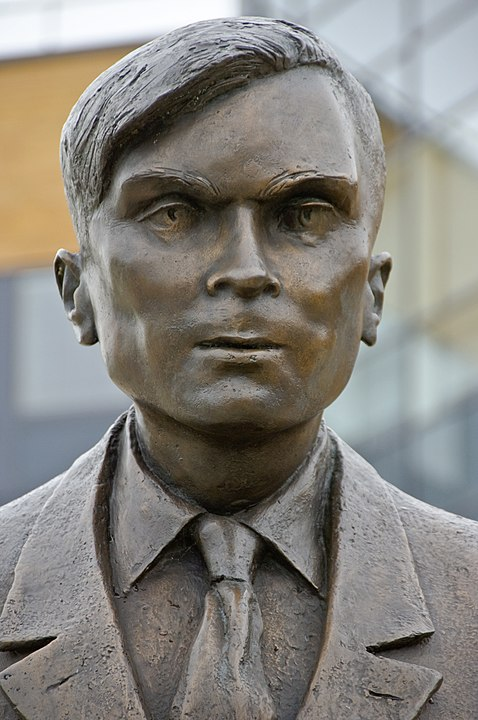
\includegraphics[width=.5\linewidth]{bild2.jpg}
  \caption{Alan Turing}
  \label{fig:alanturing}
\end{subfigure}%
\begin{subfigure}{.45\textwidth}
  \centering
  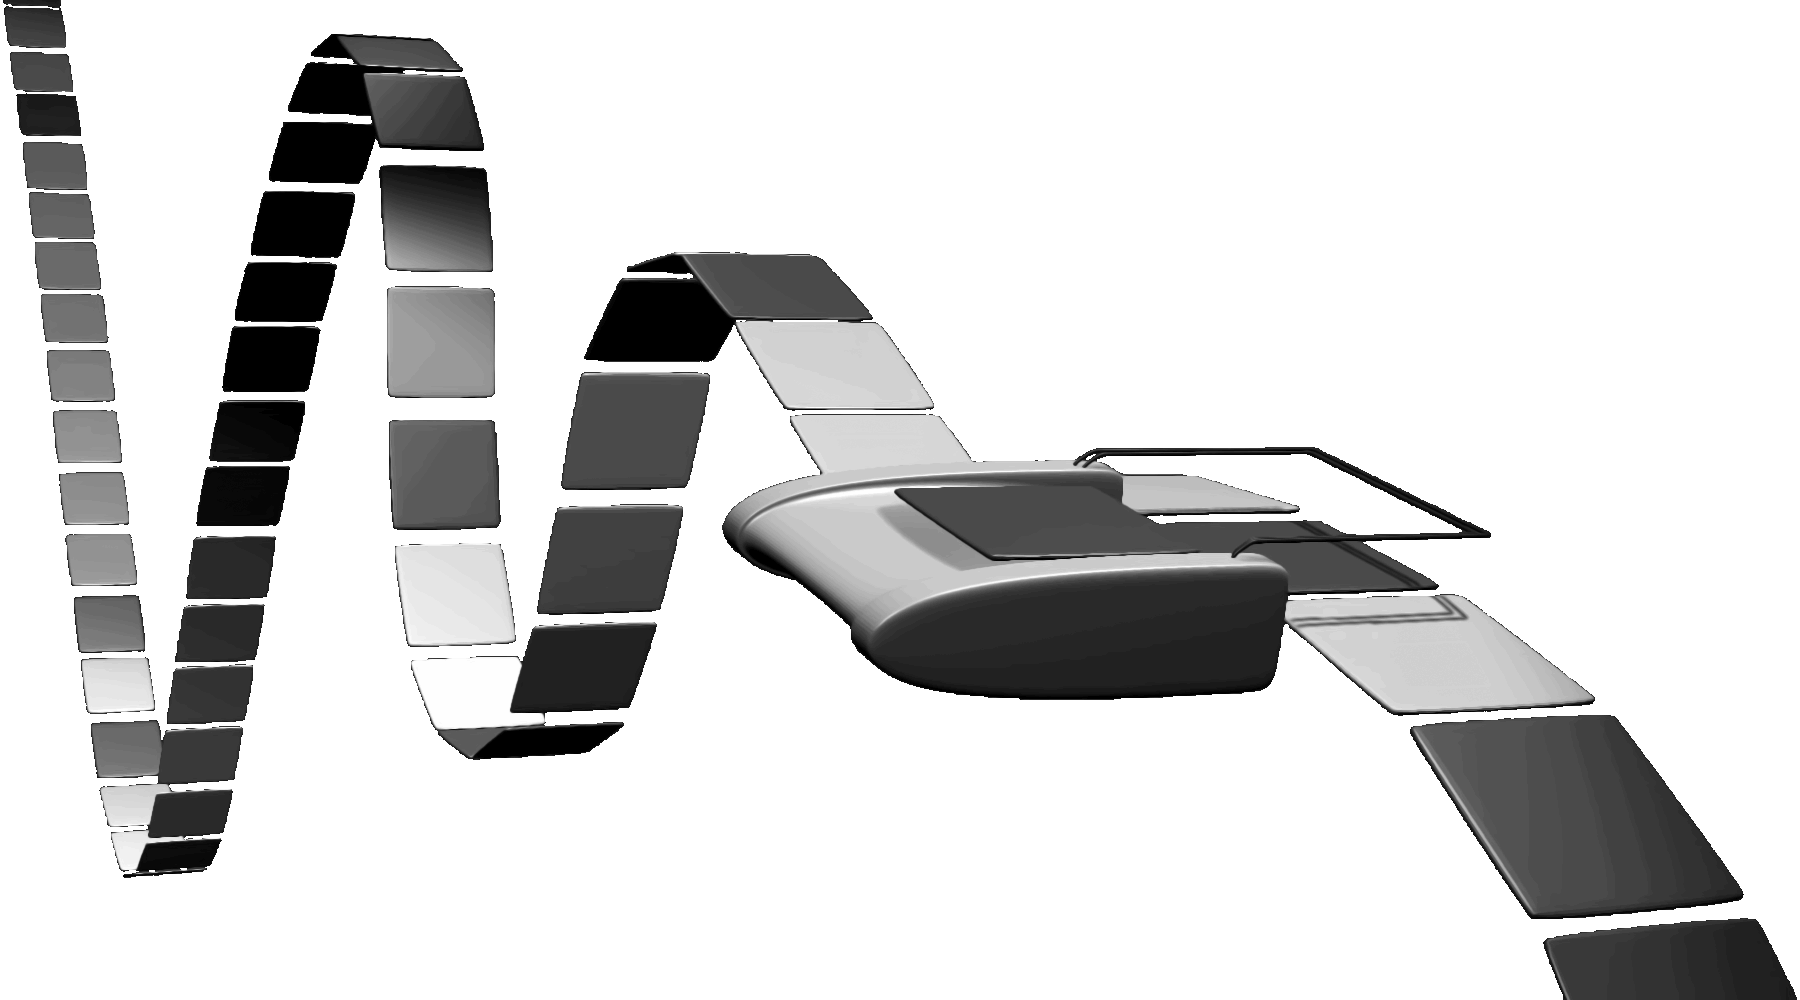
\includegraphics[width=.5\linewidth]{bild3.png}
  \caption{Turingmaschine}
  \label{fig:turingmaschine}
\end{subfigure}
\label{fig:test}
\caption{bild2.jpg und bild3.png in einer \texttt{figure}-Umgebung}
\end{figure}

Vor dem Austin Pearce Building steht eine Statue von Alan Turing (siehe Abbildung~\ref{fig:alanturing}), der als der 'Vater der Informatik' gilt. Turing verbrachte seine frühen Jahre in der Ennismore Avenue in Guildford. Er war ein brillanter britischer Mathematiker, Logiker und Informatiker, der im 20. Jahrhundert lebte. Geboren im Jahr 1912, trug er entscheidend zur Entwicklung der modernen Informatik bei und wird oft als der "Vater der Informatik" bezeichnet. \\
\\
Eines seiner bahnbrechenden Konzepte war die Turingmaschine (siehe Abbildung~\ref{fig:turingmaschine}), eine theoretische Vorstellung einer universellen Rechenmaschine. Turing entwickelte dieses abstrakte Konzept, um mathematisch zu zeigen, dass es möglich ist, mit einer einzigen Maschine jede berechenbare Funktion durchzuführen. Die Turingmaschine besteht aus einem unendlich langen Band, auf dem Symbole geschrieben werden können, und einem Kopf, der über das Band liest und schreibt. \\
\\
Während des Zweiten Weltkriegs spielte Turing eine entscheidende Rolle bei der Entschlüsselung der deutschen Enigma-Verschlüsselung, was als wichtiger Beitrag zum Sieg der Alliierten gilt. Nach dem Krieg setzte er seine Arbeit in der Informatik fort und trug zur Entwicklung von Programmierkonzepten und künstlicher Intelligenz bei. \\
\\
Leider wurde Turing in den 1950er Jahren aufgrund seiner Homosexualität strafrechtlich verfolgt und mit Auflagen belegt. Dies hatte tragische Auswirkungen auf sein Leben, und er verstarb 1954 im Alter von nur 41 Jahren. \\
\\
In Anerkennung seiner herausragenden Beiträge zur Informatik und seinem persönlichen Opfer wurde Alan Turing posthum rehabilitiert. Sein Vermächtnis lebt weiter, und die Turingmaschine bleibt ein fundamentales Konzept in der theoretischen Informatik. 

\newpage
\section{Hausaufgabe 5.3}

Es funktioniert die Installation von gnuplot nicht. Ich habe mir die Version 5.4.10 heruntergeladen und den Ordner MacOSX aus dem Ordner config in den src-Ordner gelegt und anschließend die configure-file laufen lassen. Anschließend lasse ich im Terminal den Befehl "make" laufen und bekommen folgenden Fehler 

\begin{lstlisting}[language=Python, label=pythoncode]

/Users/danielbading/Downloads/gnuplot-5.4.10/src/qtterminal/qt_term.cpp:51:10: fatal error: 'QtCore' file not found
#include <QtCore>
         ^~~~~~~~
1 error generated.
make[4]: *** [qtterminal/qt_term.o] Error 1
make[3]: *** [all-recursive] Error 1
make[2]: *** [all] Error 2
make[1]: *** [all-recursive] Error 1
make: *** [all] Error 2

\end{lstlisting}

Ich habe sowohl XCode installiert, als auch QT (über homebrew). Ich versuche es noch mal über Overleaf, aber mit meinem Laptop und Texmaker scheint es nicht zu funktionieren. 

\begin{figure}[H]

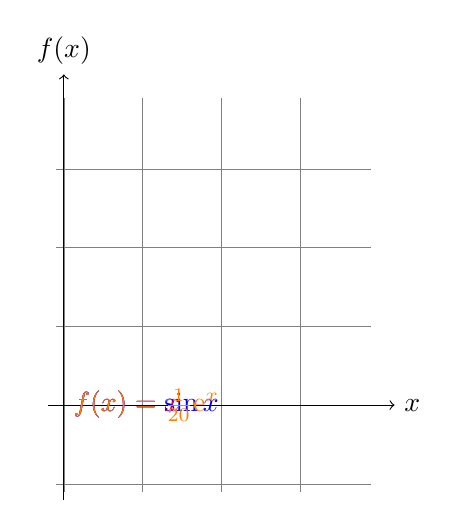
\begin{tikzpicture}[domain=0:4]
    \draw[very thin,color=gray] (-0.1,-1.1) grid (3.9,3.9);
    \draw[->] (-0.2,0) -- (4.2,0) node[right] {$x$};
    \draw[->] (0,-1.2) -- (0,4.2) node[above] {$f(x)$};
    \draw[color=red] plot[id=x] function{x} 
        node[right] {$f(x) =x$};
    \draw[color=blue] plot[id=sin] function{sin(x)} 
        node[right] {$f(x) = \sin x$};
    \draw[color=orange] plot[id=exp] function{0.05*exp(x)} 
        node[right] {$f(x) = \frac{1}{20} \mathrm e^x$};
\end{tikzpicture}

\end{figure}

\end{document}